% Created 2021-09-11 Sat 16:40
% Intended LaTeX compiler: xelatex
\documentclass[letterpaper]{article}
\usepackage{graphicx}
\usepackage{grffile}
\usepackage{longtable}
\usepackage{wrapfig}
\usepackage{rotating}
\usepackage[normalem]{ulem}
\usepackage{amsmath}
\usepackage{textcomp}
\usepackage{amssymb}
\usepackage{capt-of}
\usepackage{hyperref}
\usepackage[margin=1in]{geometry}
\usepackage{fontspec}
\usepackage{indentfirst}
\setmainfont[ItalicFont = LiberationSans-Italic, BoldFont = LiberationSans-Bold, BoldItalicFont = LiberationSans-BoldItalic]{LiberationSans}
\newfontfamily\NHLight[ItalicFont = LiberationSansNarrow-Italic, BoldFont       = LiberationSansNarrow-Bold, BoldItalicFont = LiberationSansNarrow-BoldItalic]{LiberationSansNarrow}
\newcommand\textrmlf[1]{{\NHLight#1}}
\newcommand\textitlf[1]{{\NHLight\itshape#1}}
\let\textbflf\textrm
\newcommand\textulf[1]{{\NHLight\bfseries#1}}
\newcommand\textuitlf[1]{{\NHLight\bfseries\itshape#1}}
\usepackage{fancyhdr}
\pagestyle{fancy}
\usepackage{titlesec}
\usepackage{titling}
\makeatletter
\lhead{\textbf{\@title}}
\makeatother
\rhead{\textrmlf{Compiled} \today}
\lfoot{\theauthor\ \textbullet \ \textbf{2021-2022}}
\cfoot{}
\rfoot{\textrmlf{Page} \thepage}
\titleformat{\section} {\Large} {\textrmlf{\thesection} {|}} {0.3em} {\textbf}
\titleformat{\subsection} {\large} {\textrmlf{\thesubsection} {|}} {0.2em} {\textbf}
\titleformat{\subsubsection} {\large} {\textrmlf{\thesubsubsection} {|}} {0.1em} {\textbf}
\setlength{\parskip}{0.45em}
\renewcommand\maketitle{}
\author{Houjun Liu}
\date{\today}
\title{Unit 1 Essay Planning}
\hypersetup{
 pdfauthor={Houjun Liu},
 pdftitle={Unit 1 Essay Planning},
 pdfkeywords={},
 pdfsubject={},
 pdfcreator={Emacs 27.2 (Org mode 9.4.4)}, 
 pdflang={English}}
\begin{document}

\maketitle


\section{Unit 1 Essay}
\label{sec:orga2f75df}
\subsection{General Information}
\label{sec:org193c713}
\begin{center}
\begin{tabular}{lll}
Due Date & Topic & Important Documents\\
\hline
Oct 12th & Hegemony and competition in the early modern world & Kennedy, Mann, and Friends\\
\end{tabular}
\end{center}

\subsection{Prompt}
\label{sec:org22e22b8}
\begin{html}
<!--
Cultural: Confucianism, Islam, and Christianity play varying roles in the political and economic decisions of the major regions of world (Ming/Qing, Ottomans/Mughals, Europe). \textbf{\textbf{How did culture influence the relative success of commerce and/or state formation in these regions? Was the influence positive or negative ? Were there wider ramifications?}}
Include in your essay at least two religions. Sources for: Christianity (McNeill, Kissinger), Confucianism (resources from your Kennedy essay), Islam (Bulliet, Gilbert, some Gelvin).
-->
\end{html}

Economic: The Ottomans, the Ming and Qing Empires, the Mughals and the
European kingdoms all responded to the globalization of commerce in the
early modern period in dramatically different ways. *Why did they
respond differently to the globalization of commerce and what were the
consequences?* Comparing at least two of the regions above. Gelvin
(World systems), Mann (silver), Kennedy and Arrighi might be good
general frameworks, while Bulliet (Ottomans), Gilbert (Mughals) and
McNeill (Europe) can provide some specifics.

\subsection{Documents Corner}
\label{sec:org5a16fce}
\begin{itemize}
\item @\href{KBhHIST201HomogenosceneLN.org}{KBhHIST201HomogenosceneLN}
Current day, emphasis was placed around those in native American
regions who were anti-Spanish, yet a large majority of the individuals
who really brought globalization were Spanish
\item @\href{KBhHIST201MannMing.org}{KBhHIST201MannMing} China's currency
began to show strain as Bronze prices increase whist China deals with
a botching reopening plan after closing the economy after Zheng He.
See
\href{KBhHIST201ChinasDeclineWRTReopening.org}{KBhHIST201ChinasDeclineWRTReopening}
and
\href{KBhHIST201ChinasDeclineWRTZhengHe.org}{KBhHIST201ChinasDeclineWRTZhengHe}
\item @\href{KBhHIST201Ottomans1500.org}{KBhHIST201Ottomans1500} Enjoys
control of the silk read; Huge landmass; Large army (and, large
cannons + siege trains); Strong Navy! => deployed frequently in the
Black Sea, Constantinople, North Africa

\begin{itemize}
\item Enjoyed physical control: Strategic link between Europe + Asia at
the Daranelles strait
\end{itemize}

\item @\href{KBhHIST201ProblemsWithSilver.org}{KBhHIST201ProblemsWithSilver}
--- major globalization
\end{itemize}

\subsection{Evidence bin}
\label{sec:orgdaf38d0}
\begin{itemize}
\item The Holy Roman Empire

\begin{itemize}
\item "A ruler committed to such absolute values found it impossible to
compromise, let alone to manipulate, his bargaining position."
\item Conservatism lead them directly to not compromise, getting the lower
hand
\end{itemize}

\item The Ottomans

\begin{itemize}
\item \ldots{}Established trade agreements "Such trade agreements, called
capitulations, led to European domination of Ottoman seaborne trade.
\ldots{} Far from seeing Europe as the enemy that would eventually
dismantle the empire, the Istanbul elite experimented with European
clothing and furniture styles"
\item New styles infiltrated the government causing a lack of response or
even capitulation
\end{itemize}

\item The French

\begin{itemize}
\item "Though privately religious, Richlieu viewed his duties as minister
in entirely secular terms. \ldots{} 'The state has no immortality, its
salvation is now or never.' In other words, states do not receive
credit in any world for doing what is right; they are only rewarded
for being strong enough to do what is necessary."
\item French took the stance of absolute logic and assertion of contr
\end{itemize}

\item Ming

\begin{itemize}
\item Tried to assert control --- "Northwestern Foreigners are
recalcitrant and their greed knows no bounds. I do not think our
present trade with them will ensure us a century of peace. \ldots{} As to
the foreigners in the southeast, their goods are useful to us just
as ours are to them. To use what one has to exchange for what one
does not have is what trade is all about. Moreover, these foreigners
trade with China under the name of tributary contributions. That
means China's authority is established and the foreigners are
submissive"
\item Pick and choose the outcomes only to establish authority
\end{itemize}
\end{itemize}

\subsection{Claim Synthesis}
\label{sec:orgb43a085}
\subsubsection{Development phase -- How and So-What}
\label{sec:org6de1dee}
\begin{itemize}
\item Orthodoxy on religion => non-compromise
\item New styles infiltrated the government => a lack of response or even
capitulation => overeliance on multicultralism
\item Absolute logic and assertion => overpower and compensation
\item Assertion of control => internal collapse => over-reliance on
globalization
\end{itemize}

Musing:

\begin{itemize}
\item Attempting to reach world hegemony in a multiculturalistic state will
cause eventual economic infiltration and a loss of identity, whereas
reliance on unification and control to achieve hegemony will result in
economic implosion and loss of control.
\item So\ldots{} Per Arrigi

\begin{itemize}
\item A "territorialist model" => economic implosion

\begin{itemize}
\item Ming w/ the Mann
\end{itemize}

\item A "capitalist model" => economic infiltration
\end{itemize}
\end{itemize}

\textbf{If you too multicultural, you may end up loosing your economic control.
Empires are trying to include all these cultures in one territory.}

The Ottomans, for instance, Established trade agreements "Such trade
agreements, called capitulations, led to European domination of Ottoman
seaborne trade. \ldots{} Far from seeing Europe as the enemy that would
eventually dismantle the empire, the Istanbul elite experimented with
European clothing and furniture styles" => new styles infiltrated the
government causing a lack of response or even capitulation (Bulliet)

\textbf{If you tried to overly unify your cultural identity, you may end up
loosing your civil control.}

Mughals => tried model of unity --- loosing support of Hindu nobels "The
combination of anti-Hindu policy and sentiment at court and the
reduction in the value of subsidies or land grants to Maratha mansab
dars turned Shivaji into not merely a rebel but a rival." => causing the
series of decline that the Mughals saw initiated with the Maratha
rebelion.

\textbf{If you try to, instead, exercise balance and raíson de'etat, happiness
to everyone!}

English example => "England's policy was based on throwing its weight as
the occasion required to the weaker and more threatened side to redress
the equilibrium. \ldots{} England was the one European country whose raison d
'etat did not require it to expand in Europe. Perceiving its national
interest to be in the preservation of the European balance"

And yes, there is a point where Raison de etat turns into
territorialism. But, that becomes no longer Raison de etat, that's a
tour de force: ” Richelieu's raison d'etat threatens self- destructive
tours de force\ldots{}. But Louis XN gained no peace of mind from security;
he saw in it an opportunity for conquest. In his overzealous pursuit of
raison d'etat, LouisXN alarmed the rest of Europe and brought together
an anti-French coalition which, in the end, thwarted his design.”

\subsection{Defluffifying}
\label{sec:org871fb24}
\begin{itemize}
\item If you too multicultural, you may end up loosing your economic
control. Empires are trying to include all these cultures in one
territory.
\item If you tried to overly unify your cultural identity, you may end up
loosing your civil control
\item If you try to, instead, exercise balance and raíson de'etat, happiness
to everyone!
\end{itemize}

So what? So be the third thing.

Now, defluffify by re-writing the three points + so what in as little
words as possible.

*When attempting to reach world system hegemony, over-extension of
multiculturalism will bring forth a lack of economic control whereas
over-unification of cultural identity will cause losses in civic
control; to achieve hegemony without losses in control, a state has to
exercise principles of raíson de 'etat in a position of moderation
instead of dominance.*

\begin{figure}[htbp]
\centering
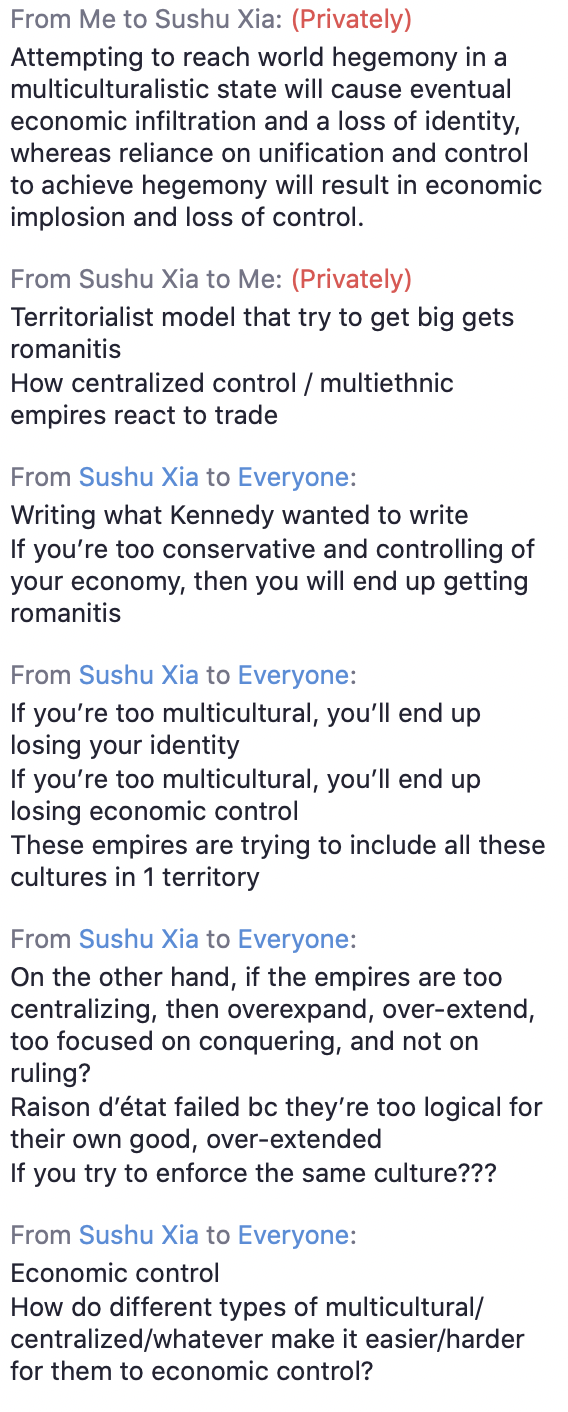
\includegraphics[width=.9\linewidth]{Screen Shot 2020-10-02 at 10.11.57 AM.png}
\caption{Screen Shot 2020-10-02 at 10.11.57 AM.png}
\end{figure}
\end{document}
